\section{Experimental Evaluation}
\label{sec:exp_evaluation}
In this section, we present the experiments conducted to empirically demonstrate that our approach not only achieves higher utility but also maintains a stronger level of privacy compared to traditional local differential privacy (LDP) protocols such as RAPPOR (Section \ref{sec:rappor}), L-OSUE (Section \ref{sec:losue}), and LOLOHA (Section \ref{sec:loloha}). We implemented our solution in Python, including our partitioning strategy and protocols. \looseness=-1
% 
\subsection{Experimental Setup}
We evaluate our approach using two synthetic datasets created for this study and two real-world mobility datasets. The synthetic datasets simulate user movement within a 100 km$^2$ area and allow us to assess behavior under contrasting spatial distributions.  
\begin{itemize}
    \item \textbf{S1}: Users are distributed uniformly across the region.
    \item \textbf{S2}: Users follow a normal distribution centered in the region.
\end{itemize}

Each synthetic dataset simulates 10,000 users moving at a constant speed of 40 km/h, generating one location report per minute over 40 timestamps. Locations are constrained by the speed to ensure realistic trajectories.

The \textbf{GeoLife} dataset\footnote{\url{https://www.microsoft.com/en-us/download/details.aspx?id=52367}} contains GPS trajectories from 183 users in Beijing. We extracted 6,261 trajectories of 20 timestamps each.  
The \textbf{Porto} dataset\footnote{\url{https://www.kaggle.com/datasets/crailtap/taxi-trajectory?select=train.csv}} comprises data from 442 taxis in Porto, Portugal. We selected 10,000 trajectories, also with 20 timestamps. Table~\ref{tab:datasets} summarizes all datasets. 

We acknowledge the use of only two real-world datasets, a limitation imposed by the scarce availability of longitudinal datasets with precise coordinate data — a key requirement for our analysis. Nevertheless, the selected datasets offer meaningful and representative insights. \looseness=-1
% 
\begin{table}[tb]
\centering
\caption{Summary of Datasets Used in the Experiments}
% \scriptsize
\begin{tabular}{l|c|c|c}
\toprule
\textbf{Dataset} & \textbf{Type} & \textbf{Distribution} & \textbf{\#Trajectories} \\
\midrule
S1 & Synthetic & Uniform & 10,000  \\
S2 & Synthetic & Normal & 10,000  \\
GeoLife & Real-world & Real-world & 6,281  \\
Porto & Real-world & Real-world & 10,000  \\
\bottomrule
\end{tabular}
\label{tab:datasets}
\end{table}
% 
For each dataset, we simulate users submitting anonymized location reports using longitudinal LDP protocols. These reports are used to estimate cell frequencies over a uniform grid. We compare these results with those obtained using ALOG's three variations (ALOG-2R, ALOG-1R-a, and ALOG-1R-b) under identical conditions. \looseness=-1

\textit{Data Utility:}  
To assess utility, we compute the \textbf{Root Mean Squared Error (RMSE)} between the true and estimated frequency distributions over time. Let \( F_i = \{f_0, \dots, f_{|G_i|}\} \) and \( \hat{F}_i = \{\hat{f}_0, \dots, \hat{f}_{|G_i|}\} \) denote the true and estimated frequencies at timestamp \( t_i \). The utility error is defined as:
% 
\begin{equation}
\small
\label{eq:utility_error}
\text{Utility Error} = \frac{1}{|T|} \sum_{i=1}^{|T|} \sqrt{ \frac{1}{|G_i|} \sum_{j=0}^{|G_i|-1} (f_j - \hat{f}_j)^2 }
\end{equation}
% 
This metric captures the accuracy of frequency estimates over time and across different spatial distributions.

% \textit{Budget Consumption:}  
% We also evaluate the \textbf{privacy budget} consumption of each method. For each timestamp \( t_i \), the budget consumed is at most \( \epsilon_\infty \) during anonymization. The total budget is:

% \[
% \text{Total Budget Consumption} = \sum_{i=1}^{|T|} \epsilon_\infty
% \]

% We report the average total budget per user to capture the cumulative privacy cost across the experiment.

\textit{Budget Consumption:}  
We also evaluate the \textbf{privacy budget} consumption of each method. For each timestamp \( t_i \), the budget consumed is at most \( \epsilon_\infty \) during anonymization. The total budget consumption is: $\sum_{i=1}^{|T|} \epsilon_\infty$. We report the average total budget per user to capture the cumulative privacy cost across the experiment.



\subsection{Results}

\paragraph{Grid Granularity x Utility:}first, we analyze the adjustment of grid granularity, which is a key aspect of the proposed adaptive longitudinal grid framework. Specifically, we compare methods using static uniform grids with ALOG, starting from the same initial grid granularity. The relationship between grid granularity and data utility is central to understanding how the system adapts to different data distributions while balancing privacy constraints.


\definecolor{sn1}{rgb}{0.00392156862745098, 0.45098039215686275, 0.6980392156862745}
\definecolor{sn2}{rgb}{0.8705882352941177, 0.5607843137254902, 0.0196078431372549}
\definecolor{sn3}{rgb}{0.00784313725490196, 0.6196078431372549, 0.45098039215686275}
\definecolor{sn4}{rgb}{0.8352941176470589, 0.3686274509803922, 0.0}
\definecolor{sn5}{rgb}{0.8, 0.47058823529411764, 0.7372549019607844}
\definecolor{sn6}{rgb}{0.792156862745098, 0.5686274509803921, 0.3803921568627451}

\begin{figure}[tb] 
    \centering
    \Description{Granularity Plots}
    \begin{tikzpicture}
        \begin{axis}[
        hide axis,
        xmin=0, xmax=1,
        ymin=0, ymax=1,
        legend style={
            draw=none,
            inner sep=0,outer sep=0,
            column sep=.5ex, % Adjust spacing between columns
            legend columns=3, % Number of legend items per row
            at={(0.5,0)}, % Position legend below the axis
            anchor=south
        },
        width=\columnwidth % Fit within one column
        ]
            % ALOG-1R-a: diagonal lines pattern
            \addplot[
            pattern=north east lines,
            pattern color=sn1,
            area legend
            ] coordinates {(0,0)};
            \addlegendentry{ALOG-1R-a}
    
            % ALOG-1R-b: crosshatch pattern
            \addplot[pattern=north west lines, pattern color=sn2, area legend] 
                coordinates {(0,0)};
            \addlegendentry{ALOG-1R-b}
    
            % ALOG-2R: grid pattern
            \addplot[pattern=vertical lines, pattern color=sn3, area legend] 
                coordinates {(0,0)};
            \addlegendentry{ALOG-2R}
    
            % RAPPOR: solid red color with no pattern
            \addplot[fill=black, fill=sn6, draw=none, area legend] 
                coordinates {(0,0)};
            \addlegendentry{RAPPOR}
            
            % LOSUE: diagonal crosshatch pattern
            \addplot[pattern=crosshatch, pattern color=sn5, area legend] 
                coordinates {(0,0)};
            \addlegendentry{LOSUE}
    
            % LOLOHA: horizontal lines pattern
            \addplot[pattern=horizontal lines, pattern color=sn4, area         legend] 
                 coordinates {(0,0)};
            \addlegendentry{LOLOHA}
        \end{axis}
    \end{tikzpicture}

    \centering
    % First sequence
    \begin{subfigure}{0.49\textwidth} % Adjust subfigure size to fit single column
        \centering
        \begin{minipage}{0.80\textwidth}
            \centering
            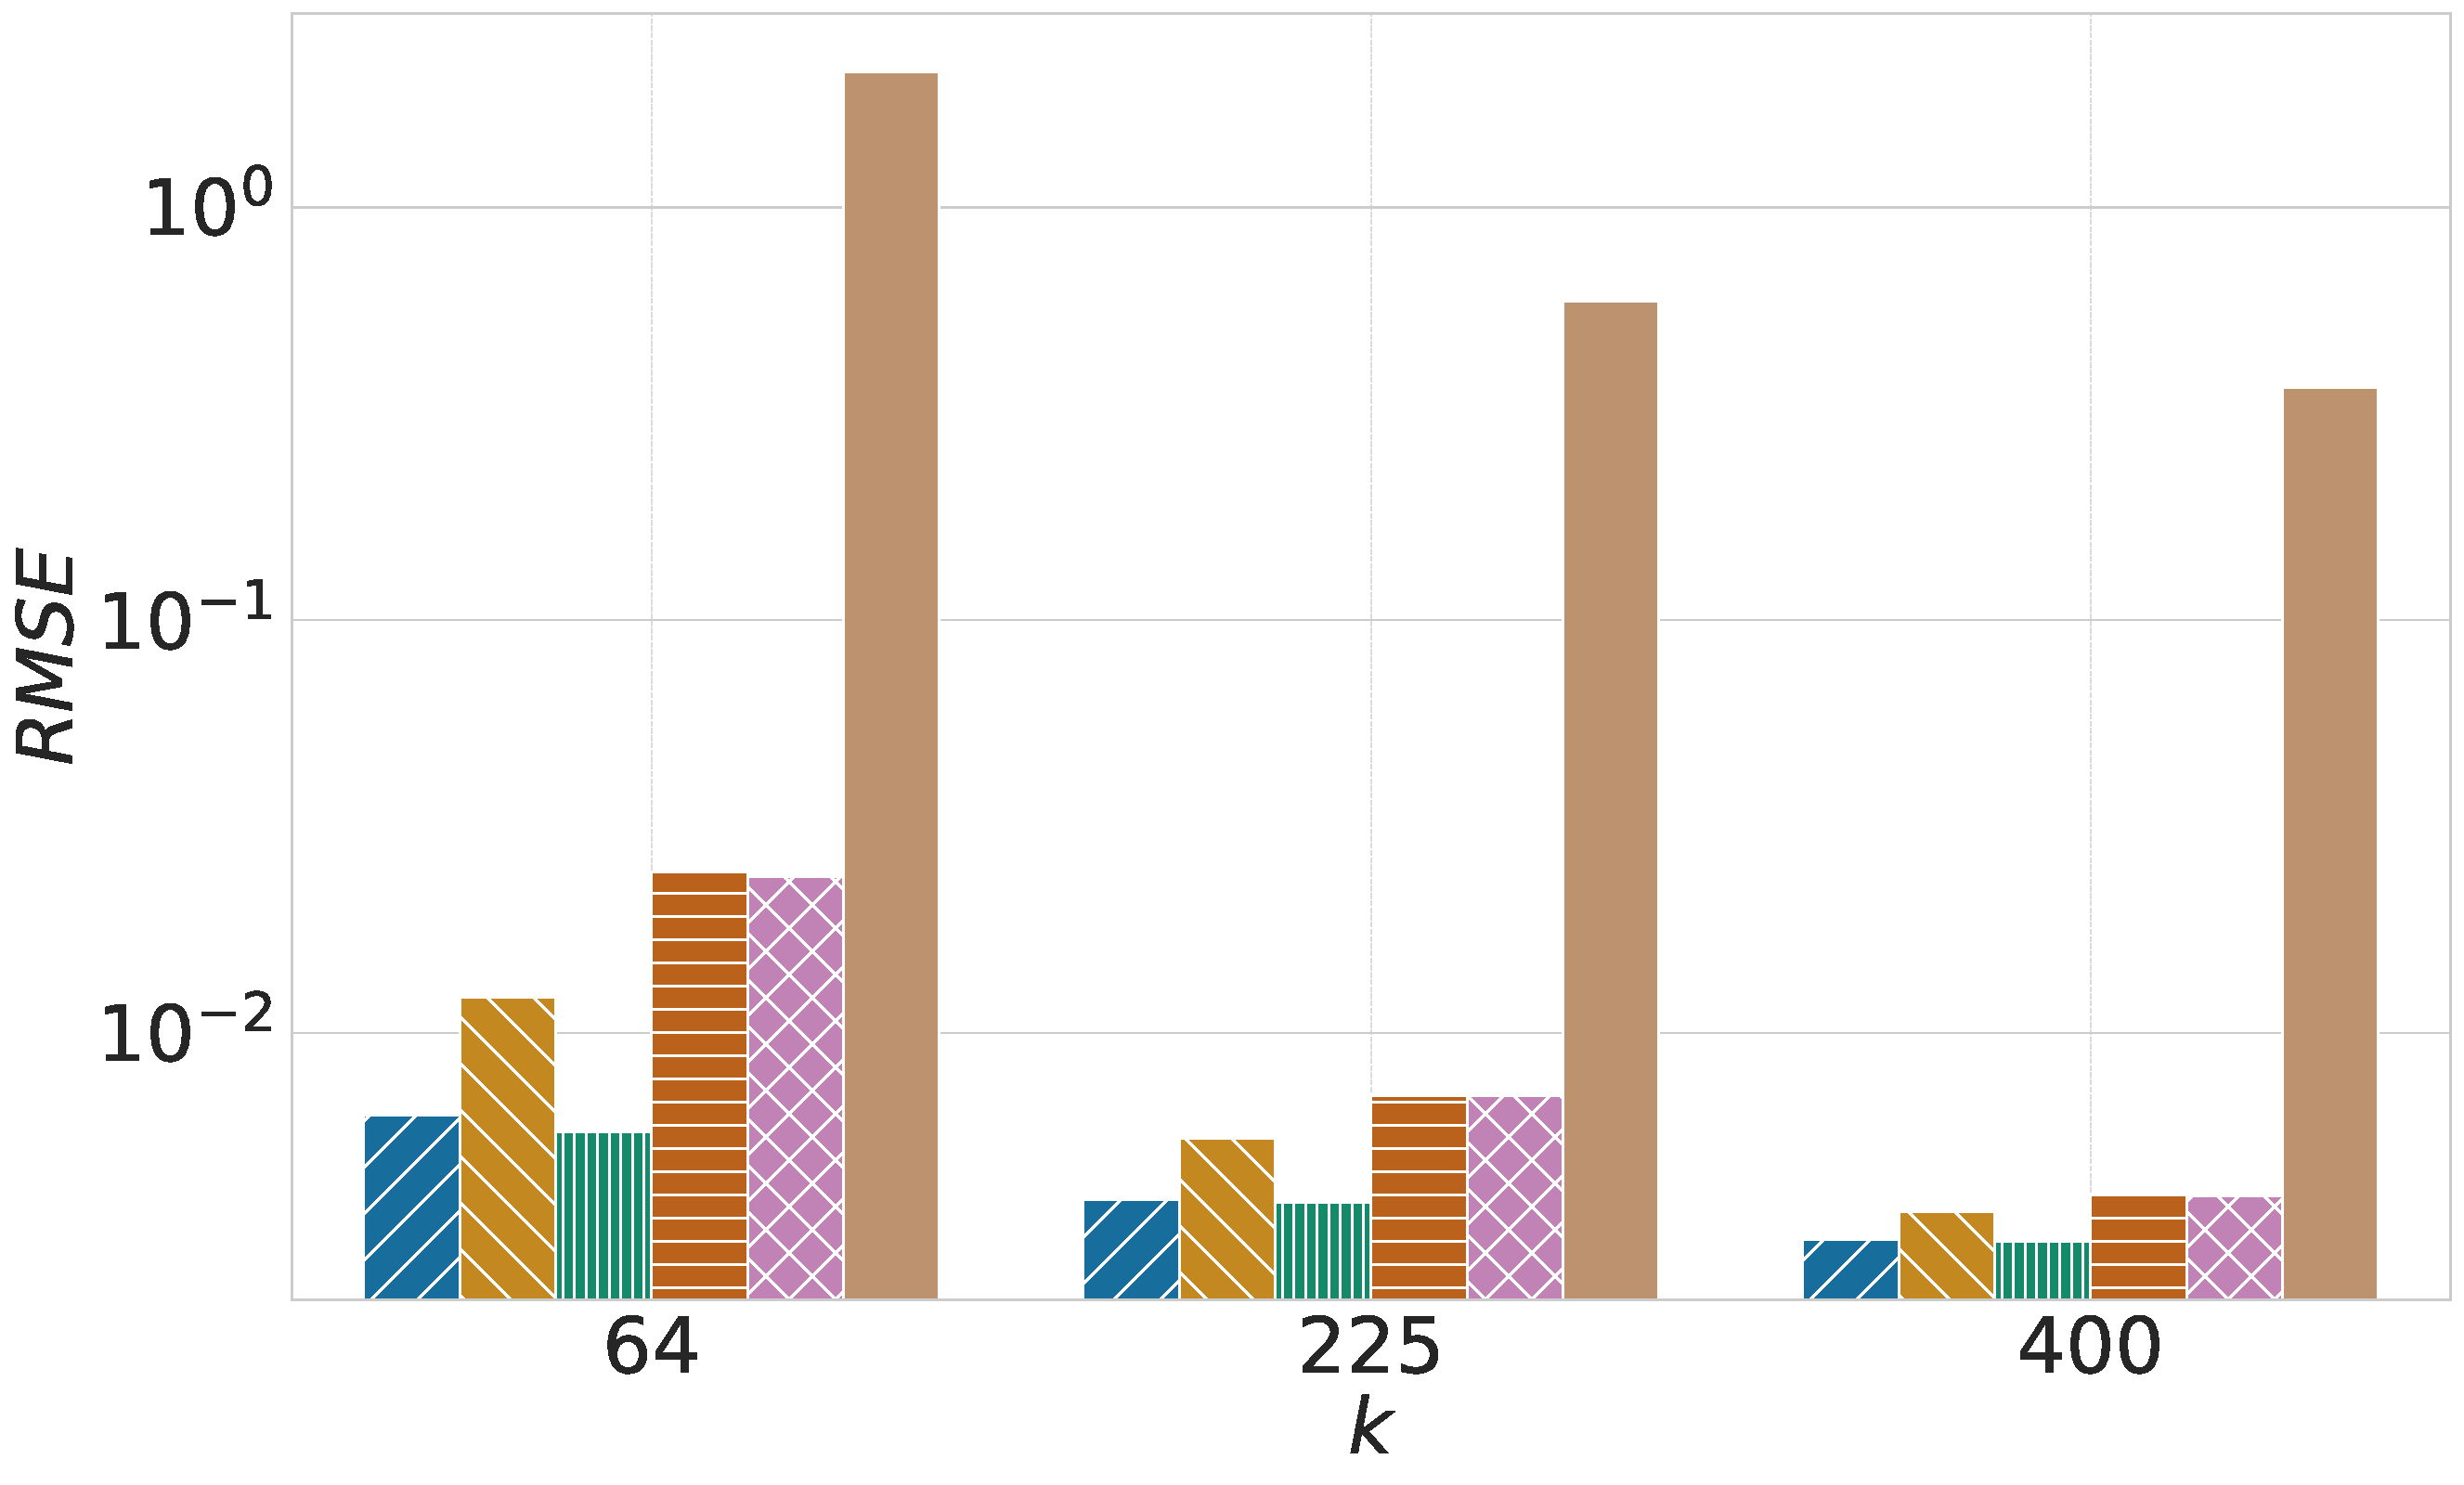
\includegraphics[width=\linewidth]{sections/figures/K_RMSE_BAR/rmse_compare_0.1_grid_avg_barchart_uniform.pdf}
            \caption{S1 with $\epsilon_{\infty}=0.1$}        
            \label{fig:granularity_s1}
        \end{minipage}
        \hfill
        \begin{minipage}{0.80\textwidth}
            \centering
            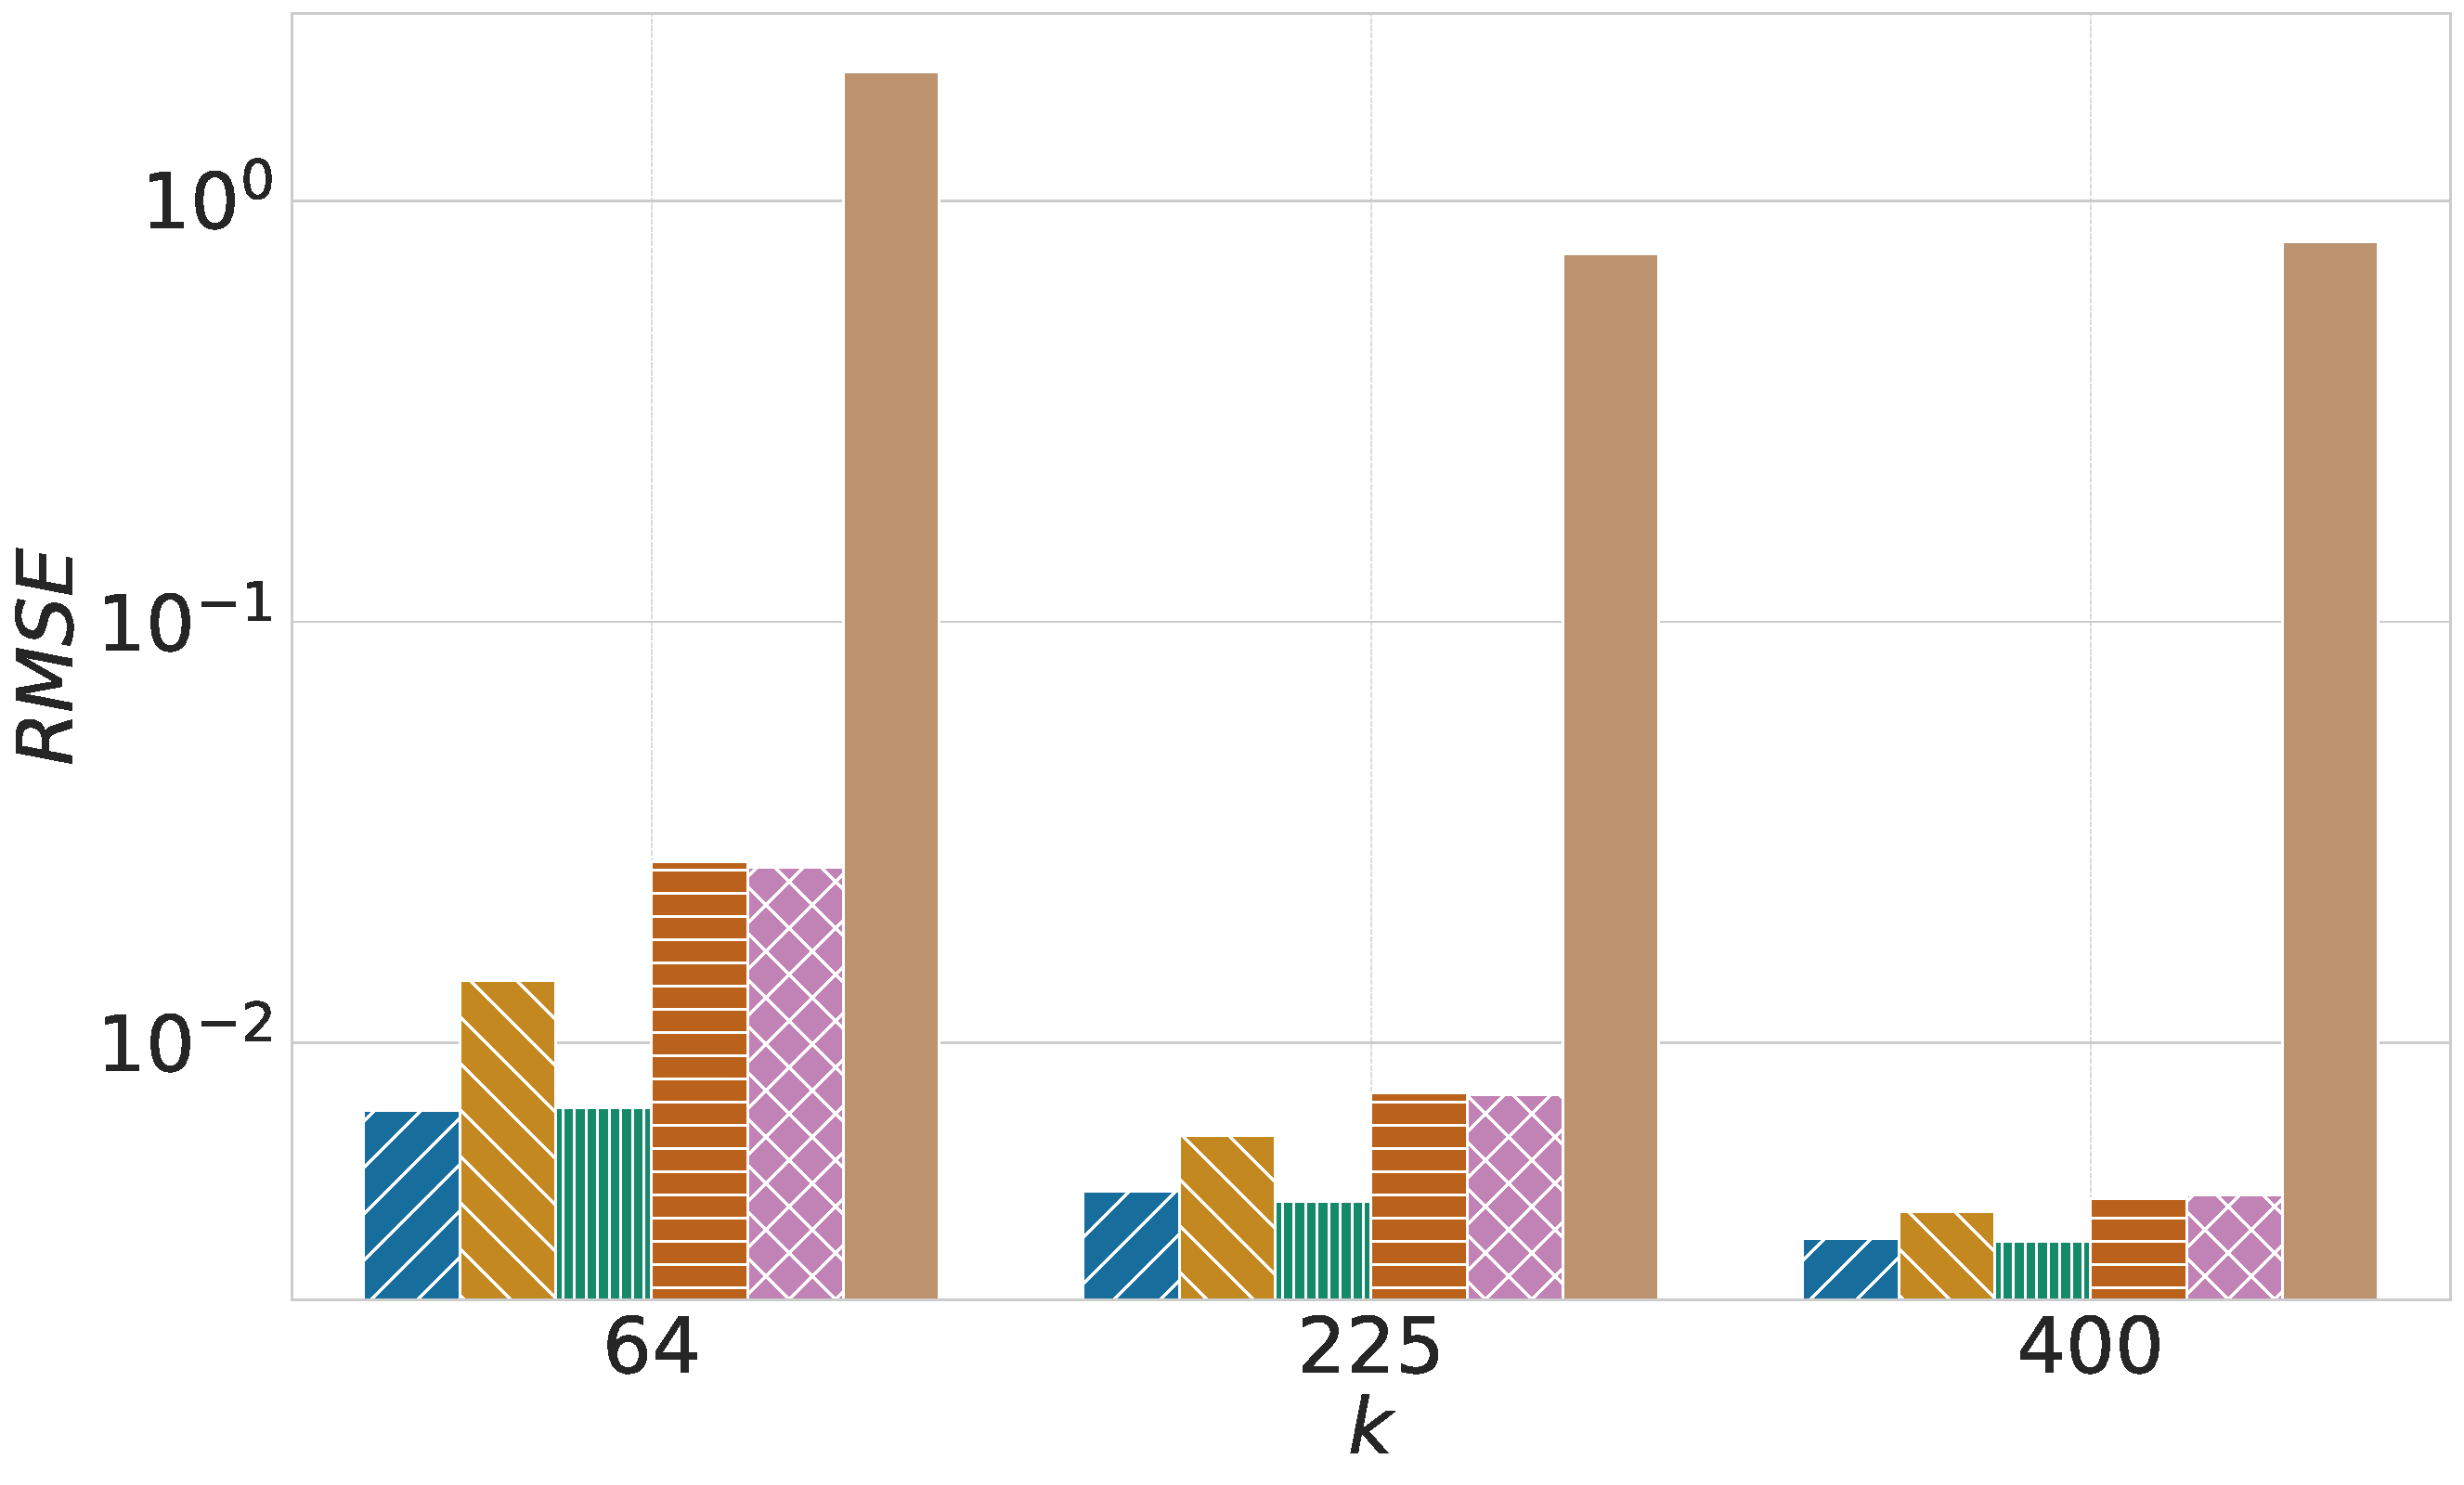
\includegraphics[width=\linewidth]{sections/figures/K_RMSE_BAR/rmse_compare_0.1_grid_avg_barchart_normal.pdf}
            \caption{S2 with $\epsilon_{\infty}=0.1$}
            \label{fig:granularity_s2}
        \end{minipage}
        \label{fig:sequence1}
    \end{subfigure}
    
    
    % Second sequence
    \begin{subfigure}{0.49\textwidth} % Adjust subfigure size to fit single column
        \centering
        \begin{minipage}{0.8\textwidth}
            \centering
            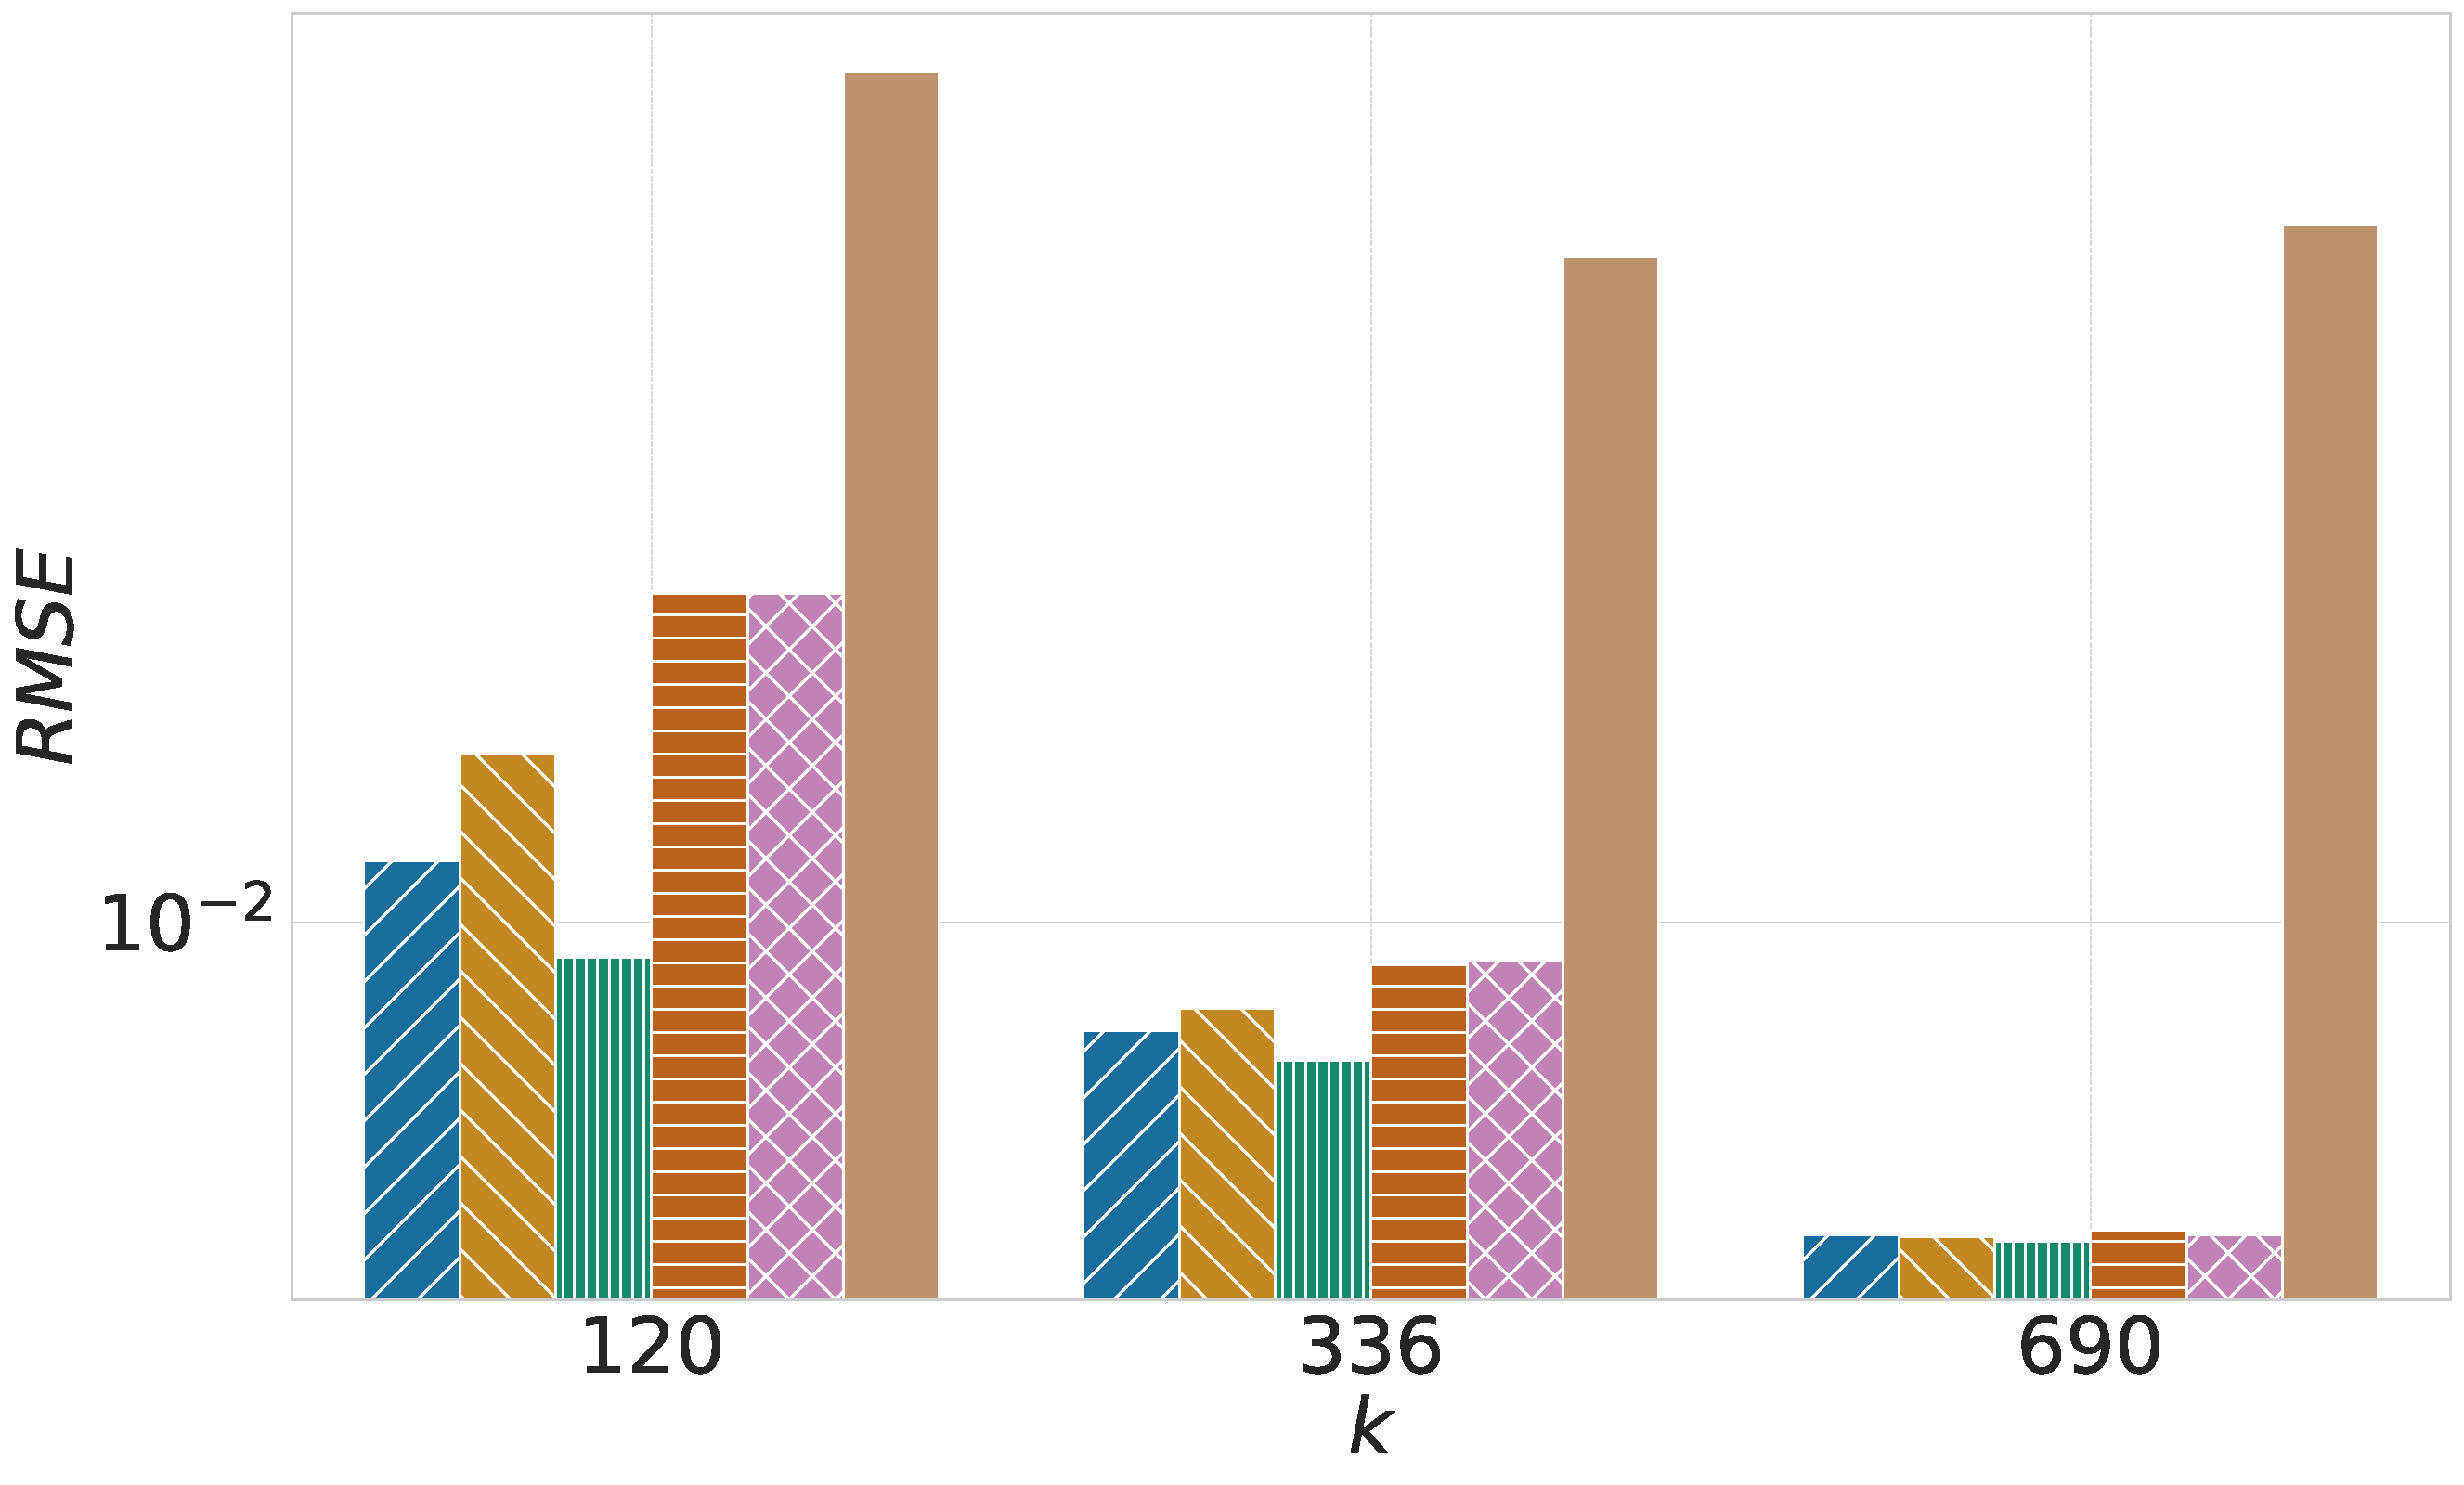
\includegraphics[width=\linewidth]{sections/figures/K_RMSE_BAR/rmse_compare_0.3_grid_avg_barchart_geo.pdf}
            \caption{Geolife with $\epsilon_{\infty}=0.3$}
            \label{fig:granularity_geo}
        \end{minipage}
        \hfill
        \begin{minipage}{0.8\textwidth}
            \centering
            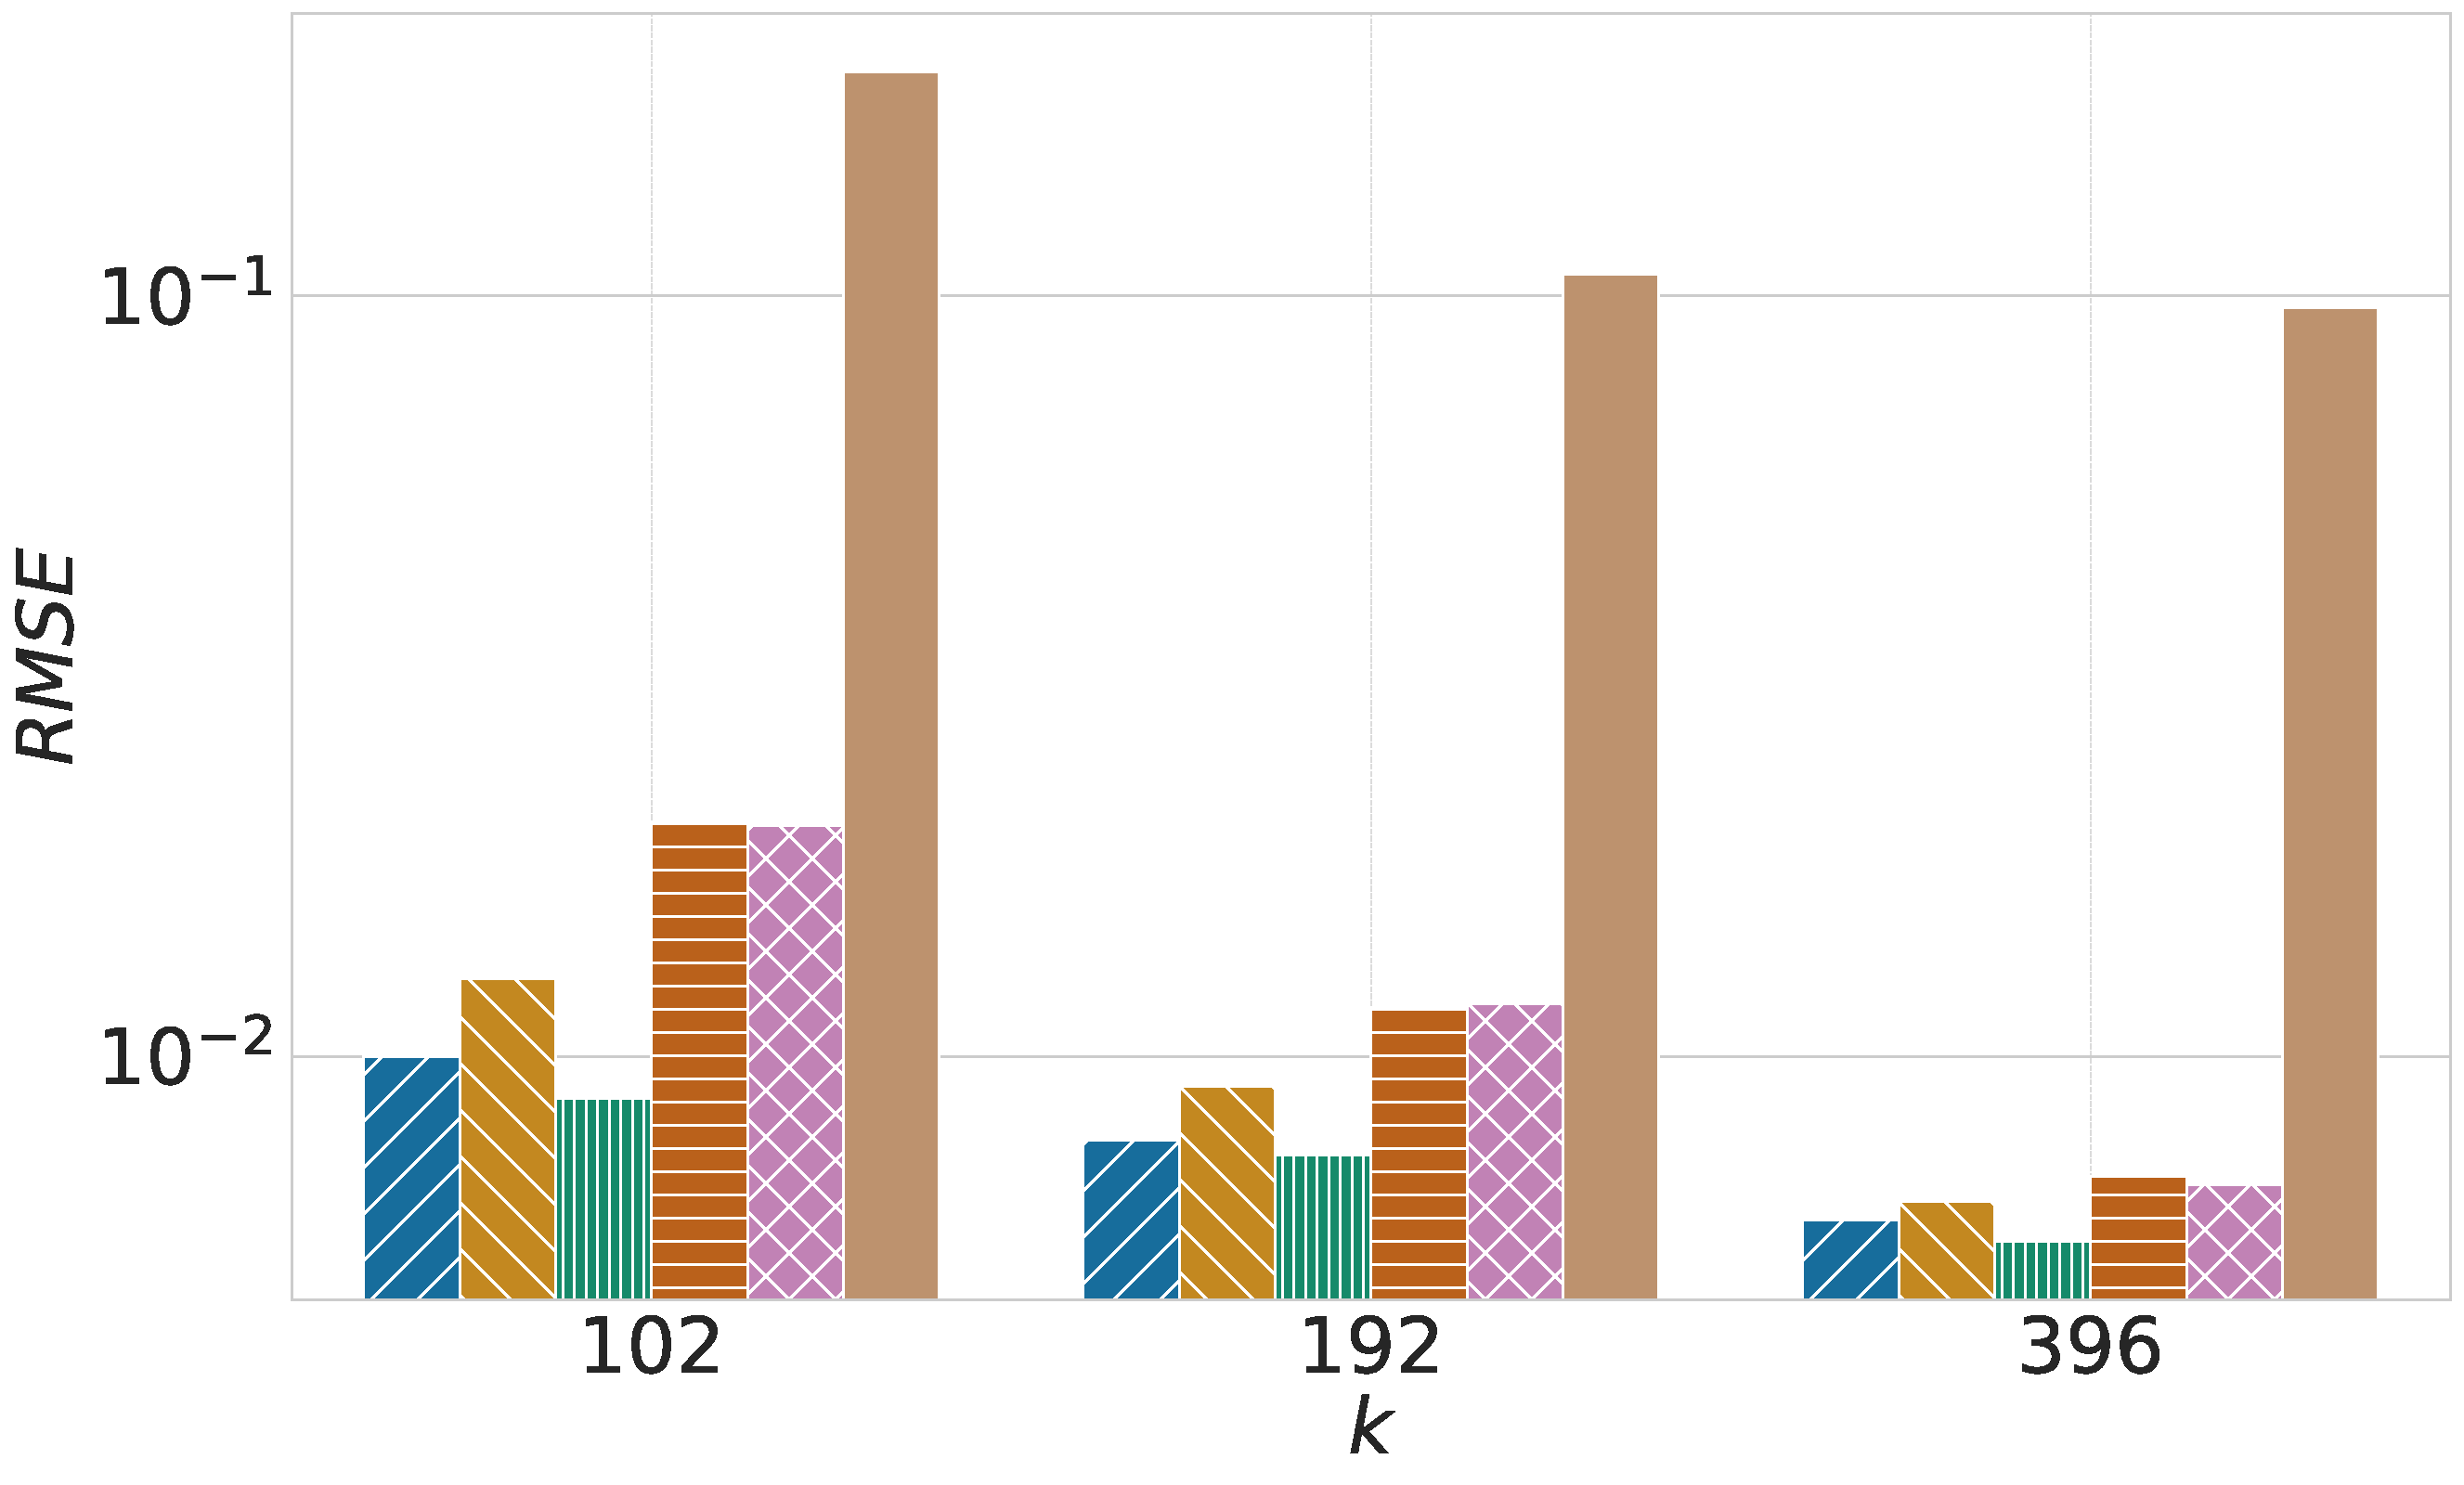
\includegraphics[width=\linewidth]{sections/figures/K_RMSE_BAR/rmse_compare_0.3_grid_avg_barchart_porto.pdf}
            \caption{Porto with $\epsilon_{\infty}=0.3$}
            \label{fig:granularity_porto}
        \end{minipage}
        \label{fig:sequence2}
    \end{subfigure}
    \caption{RMSE variation as a function of grid size for the four datasets: S1, S2, GeoLife, and Porto. Each chart represents the
error in data analysis when the initial grid size is set.}
\label{fig:granularity_barchart}
\end{figure}
Theoretically, the expected utility of each ALOG variant is influenced by the trade-off between noise magnitude (from LDP perturbation) and the granularity of the grid. According to the variance of LDP frequency estimation protocols such as LOSUE, the estimation variance is inversely proportional to the number of reports per grid cell. Thus uniform grid approaches (e.g., RAPPOR) are expected to exhibit higher error in regions with skewed data distributions due to non-uniformity error.

Figure \ref{fig:granularity_barchart} illustrates the effectiveness of our proposed adaptive grid approaches in enhancing utility compared to uniform grid-based methods, which consistently yielded the highest $RMSE$ across all scenarios. On the x-axis of the figure, $k$ represents the number of cells in the grid, while the y-axis shows the $RMSE$ between the real and estimated frequencies. Among the adaptive grid strategies, ALOG-2R emerged as the most effective, achieving the lowest $RMSE$ due to its two-round mechanism. In contrast, the ALOG-1R-b method demonstrated the poorest performance among the ALOG approaches. This is attributed to its reliance on a fixed base grid size during the grid adaptation process, which results in the loss of previously acquired knowledge and compromises its utility. For this experiment, a permanent privacy budget of 0.1 was used for each timestamp, and the adaptation window was set to 4.

\paragraph{Privacy Budget x Utility:}analyzing the relationship between the privacy budget and utility is crucial, as it highlights the trade-off between privacy guarantees and the accuracy of data estimates. A well-calibrated privacy budget establishes a balance, minimizing the $RMSE$ while ensuring adequate privacy protection. This balance is essential for practical deployments in applications involving sensitive data. \looseness=-1

In our experiments, we varied the privacy budget values between 0 and 1, with the budget representing the upper bound of privacy for each individual. We set up a cell size of $700 \, \text{meters} \times 700 \, \text{meters} $, which results in an initial grid granularity of $k = 225$ for datasets S1 and S2, $k = 336$ for Geolife, and $k = 192$ for Porto. The grid adaptation window was set to $w = 4$ moments of time. This setup allows us to explore how different privacy levels affect the utility of the system while maintaining the required privacy guarantees, as shown in Table \ref{tab:mse_budge}.


In the S1 and S2 datasets, ALOG-2R consistently achieves the lowest $RMSE$ values for all privacy budgets. This demonstrates how the two-stage model effectively enhances utility while maintaining compliance with privacy requirements. ALOG-1R-a follows closely, with slightly higher $RMSE$ values than ALOG-2R but significantly outperforming ALOG-1R-b.

The LOLOHA and LOSUE methods, while maintaining relatively stable performance across datasets, generally exhibit higher $RMSE$ values compared to ALOG-2R. Notably, RAPPOR, despite being a widely used method for privacy preservation, demonstrates the highest $RMSE$ values, particularly in scenarios with small privacy budgets, indicating its limitations in achieving high utility.

For the Geolife and Porto datasets, a similar pattern emerges. ALOG-2R continues to outperform other methods, achieving the best balance between privacy and utility. In the Geolife dataset, the $RMSE$ for ALOG-2R is consistently the lowest, especially for $\epsilon = 0.05$ and $\epsilon = 0.5$. In the Porto dataset, ALOG-2R again achieves the best results, with noticeable improvements over LOLOHA and LOSUE.  \looseness=-1 %This consistency across diverse datasets highlights the robustness of ALOG-2R as an adaptive grid method.

In summary, Table \ref{tab:mse_budge} emphasizes the significance of selecting an appropriate privacy budget $\epsilon$ and algorithm based on the application requirements. The results underscore the effectiveness of ALOG-2R in achieving a superior trade-off between privacy and utility, making it a strong candidate for practical deployments in sensitive data applications.

% \begin{table}[!tb]
% \centering
% \scriptsize
% \caption{RMSE ($\times 10^{-3}$) for $k=225$ in S1 and S2, $k=336$ in Geolife, and $k=192$ in Porto, with ALOG using $w=4$.}
% \begin{tabular}{c|c|cccccc}
% \toprule
% \textbf{DataSet} & \textbf{Budget}  & \textbf{ALOG-1R-a} & \textbf{ALOG-1R-b} & \textbf{ALOG-2R} & \textbf{LOLOHA} & \textbf{LOSUE} & \textbf{RAPPOR} \\
% \midrule
% \multirow{4}{*}{\textbf{S1}} 
% & $\epsilon = 0.05$ & 4.009 & 5.497 & \cellcolor{black!8}$\mathbf{3.908}$  & 6.948  & 6.924  & 1599.661  \\
% & $\epsilon = 0.1$  & 3.919  & 5.473  & \cellcolor{black!8}$\mathbf{3.866}$  & 7.124  & 6.960  & 1068.873  \\
% & $\epsilon = 0.5$  & 4.125  & 5.417  & \cellcolor{black!8}$\mathbf{3.771}$  & 6.882  & 6.884  & 153.428  \\
% & $\epsilon = 1.0$  & 3.998  & 5.406  & \cellcolor{black!8}$\mathbf{3.554}$  & 6.903  & 6.866  & 67.914  \\

% \midrule
% \multirow{3}{*}{\textbf{S2}} 
% & $\epsilon = 0.05$ & 4.314  & 5.953  & \cellcolor{black!8}$\mathbf{4.282}$  & 7.391  & 7.506  & 834.638  \\
% & $\epsilon = 0.1$  & 4.476  & 5.967  & \cellcolor{black!8}$\mathbf{4.212}$  & 7.516  & 7.536  & 666.694  \\
% & $\epsilon = 0.5$  & 4.389  & 6.009  & \cellcolor{black!8}$\mathbf{4.012}$  & 7.522  & 7.488  & 87.250  \\
% & $\epsilon = 1.0$  & 4.335  & 5.903  & \cellcolor{black!8}$\mathbf{4.102}$  & 7.749  & 7.489  & 112.595  \\
% \midrule

% \multirow{3}{*}{\textbf{Geolife}} 
% & $\epsilon = 0.05$ & 7.672  & 8.183  & \cellcolor{black!8}$\mathbf{6.694}$  & 9.053  & 9.162  & 432.922  \\
% & $\epsilon = 0.1$  & \cellcolor{black!8}$\mathbf{7.220}$  & 8.151  & 7.513  & 9.042  & 9.028  & 285.988  \\
% & $\epsilon = 0.5$  & 7.403  & 8.116  & \cellcolor{black!8}$\mathbf{6.855}$  & 9.001  & 9.190  & 77.613  \\
% & $\epsilon = 1.0$  & \cellcolor{black!8}$\mathbf{6.933}$  & 8.154  & 7.044  & 8.937  & 8.996  & 41.224  \\

% \midrule
% \multirow{3}{*}{\textbf{Porto}}
% & $\epsilon = 0.05$ & 7.522  & 9.211  & \cellcolor{black!8}$\mathbf{7.303}$  & 11.358  & 11.320  & 829.024  \\
% & $\epsilon = 0.1$  & 7.657  & 8.720  & \cellcolor{black!8}$\mathbf{7.151}$  & 11.524  & 11.831  & 197.978  \\
% & $\epsilon = 0.5$  & 7.831  & 8.796  & \cellcolor{black!8}$\mathbf{6.886}$  & 11.778  & 11.332  & 111.164  \\
% & $\epsilon = 1.0$  & 7.474  & 8.907  & \cellcolor{black!8}$\mathbf{6.876}$  & 11.704  & 11.444  & 68.865  \\

% \bottomrule
% \end{tabular}
% \label{tab:mse_budge}
% \end{table}

% \newcolumntype{L}{>{\raggedright\arraybackslash}X} % Left-aligned X column
% \newcolumntype{C}{>{\centering\arraybackslash}X}   % Centered X column
% \newcolumntype{R}{>{\raggedleft\arraybackslash}X}  % Right-aligned X column

\begin{table*}
\centering
% \small
\caption{RMSE ($\times 10^{-3}$) for $k=225$ in S1 and S2, $k=336$ in Geolife, and $k=192$ in Porto, with ALOG using $w=4$.}
\begin{tabular}{c|c|cccccc}
\toprule
\textbf{DataSet} & \textbf{Budget}  & \textbf{ALOG-1R-a} & \textbf{ALOG-1R-b} & \textbf{ALOG-2R} & \textbf{LOLOHA} & \textbf{LOSUE} & \textbf{RAPPOR} \\
\midrule
\multirow{4}{*}{\textbf{S1}} 
& $\epsilon = 0.05$ & 4.009 & 5.497 & \cellcolor{black!8}$\mathbf{3.908}$  & 6.948  & 6.924  & 1599.661  \\
& $\epsilon = 0.1$  & 3.919  & 5.473  & \cellcolor{black!8}$\mathbf{3.866}$  & 7.124  & 6.960  & 1068.873  \\
& $\epsilon = 0.5$  & 4.125  & 5.417  & \cellcolor{black!8}$\mathbf{3.771}$  & 6.882  & 6.884  & 153.428  \\
& $\epsilon = 1.0$  & 3.998  & 5.406  & \cellcolor{black!8}$\mathbf{3.554}$  & 6.903  & 6.866  & 67.914  \\

\midrule
\multirow{3}{*}{\textbf{S2}} 
& $\epsilon = 0.05$ & 4.314  & 5.953  & \cellcolor{black!8}$\mathbf{4.282}$  & 7.391  & 7.506  & 834.638  \\
& $\epsilon = 0.1$  & 4.476  & 5.967  & \cellcolor{black!8}$\mathbf{4.212}$  & 7.516  & 7.536  & 666.694  \\
& $\epsilon = 0.5$  & 4.389  & 6.009  & \cellcolor{black!8}$\mathbf{4.012}$  & 7.522  & 7.488  & 87.250  \\
& $\epsilon = 1.0$  & 4.335  & 5.903  & \cellcolor{black!8}$\mathbf{4.102}$  & 7.749  & 7.489  & 112.595  \\
\midrule

\multirow{3}{*}{\textbf{Geolife}} 
& $\epsilon = 0.05$ & 7.672  & 8.183  & \cellcolor{black!8}$\mathbf{6.694}$  & 9.053  & 9.162  & 432.922  \\
& $\epsilon = 0.1$  & \cellcolor{black!8}$\mathbf{7.220}$  & 8.151  & 7.513  & 9.042  & 9.028  & 285.988  \\
& $\epsilon = 0.5$  & 7.403  & 8.116  & \cellcolor{black!8}$\mathbf{6.855}$  & 9.001  & 9.190  & 77.613  \\
& $\epsilon = 1.0$  & \cellcolor{black!8}$\mathbf{6.933}$  & 8.154  & 7.044  & 8.937  & 8.996  & 41.224  \\

\midrule
\multirow{3}{*}{\textbf{Porto}}
& $\epsilon = 0.05$ & 7.522  & 9.211  & \cellcolor{black!8}$\mathbf{7.303}$  & 11.358  & 11.320  & 829.024  \\
& $\epsilon = 0.1$  & 7.657  & 8.720  & \cellcolor{black!8}$\mathbf{7.151}$  & 11.524  & 11.831  & 197.978  \\
& $\epsilon = 0.5$  & 7.831  & 8.796  & \cellcolor{black!8}$\mathbf{6.886}$  & 11.778  & 11.332  & 111.164  \\
& $\epsilon = 1.0$  & 7.474  & 8.907  & \cellcolor{black!8}$\mathbf{6.876}$  & 11.704  & 11.444  & 68.865  \\

\bottomrule
\end{tabular}
\label{tab:mse_budge}
\end{table*}

\paragraph{Longitudinal Setting x Utility:}another important aspect to consider is the impact of data's longitudinal nature on utility. Figure \ref{fig:longitudinality_barchart} illustrates how the temporal evolution of data affects the performance of privacy-preserving mechanisms, which is crucial for applications that involve dynamic and continuously changing datasets. Understanding this impact allows us to assess the robustness of adaptive grid methods, such as ALOG-2R, in maintaining low $RMSE$ while addressing the challenges posed by temporal variations in data distribution. This analysis will further provide insights into how privacy budgets and grid adaptations interact over time, ensuring the methods remain effective in real-world scenarios with longitudinal data.

Figure \ref{fig:longitudinality_barchart} consists of four subcharts, each corresponding to a different data set. These graphs illustrate the relationship between the number of consecutive reports sent by users and the $RMSE$. In the preceding analysis, RAPPOR consistently demonstrated significantly poorer performance compared to the other methods (as seen in Figure \ref{fig:granularity_barchart} and Table \ref{tab:mse_budge}). To provide a clearer visualization and focus on the comparative differences among the higher-performing approaches, RAPPOR was excluded from Figure \ref{fig:longitudinality_barchart}. However, it is important to note that the trend of RAPPOR's inferior performance continues in this subsequent analysis, though not shown for visual clarity. \looseness=-1

The ALOG approaches exhibit much better performance, with ALOG-2R and ALOG-1R-a showing very similar results, often achieving the lowest $RMSE$ values. These methods leverage their adaptive mechanisms to outperform not only RAPPOR but also other approaches like LOSUE and LOLOHA, which perform moderately but fail to match the precision of ALOG methods.

The consistent superiority of ALOG-2R and ALOG-1R-a across datasets highlights their adaptability and efficiency, particularly in scenarios with a higher frequency of consecutive user requests. These results underline the importance of selecting advanced adaptive grid methods to ensure low $RMSE$ in privacy-preserving systems.
% 
\begin{figure*}[!tb]
    \centering
    \Description{longitudinality plots}
    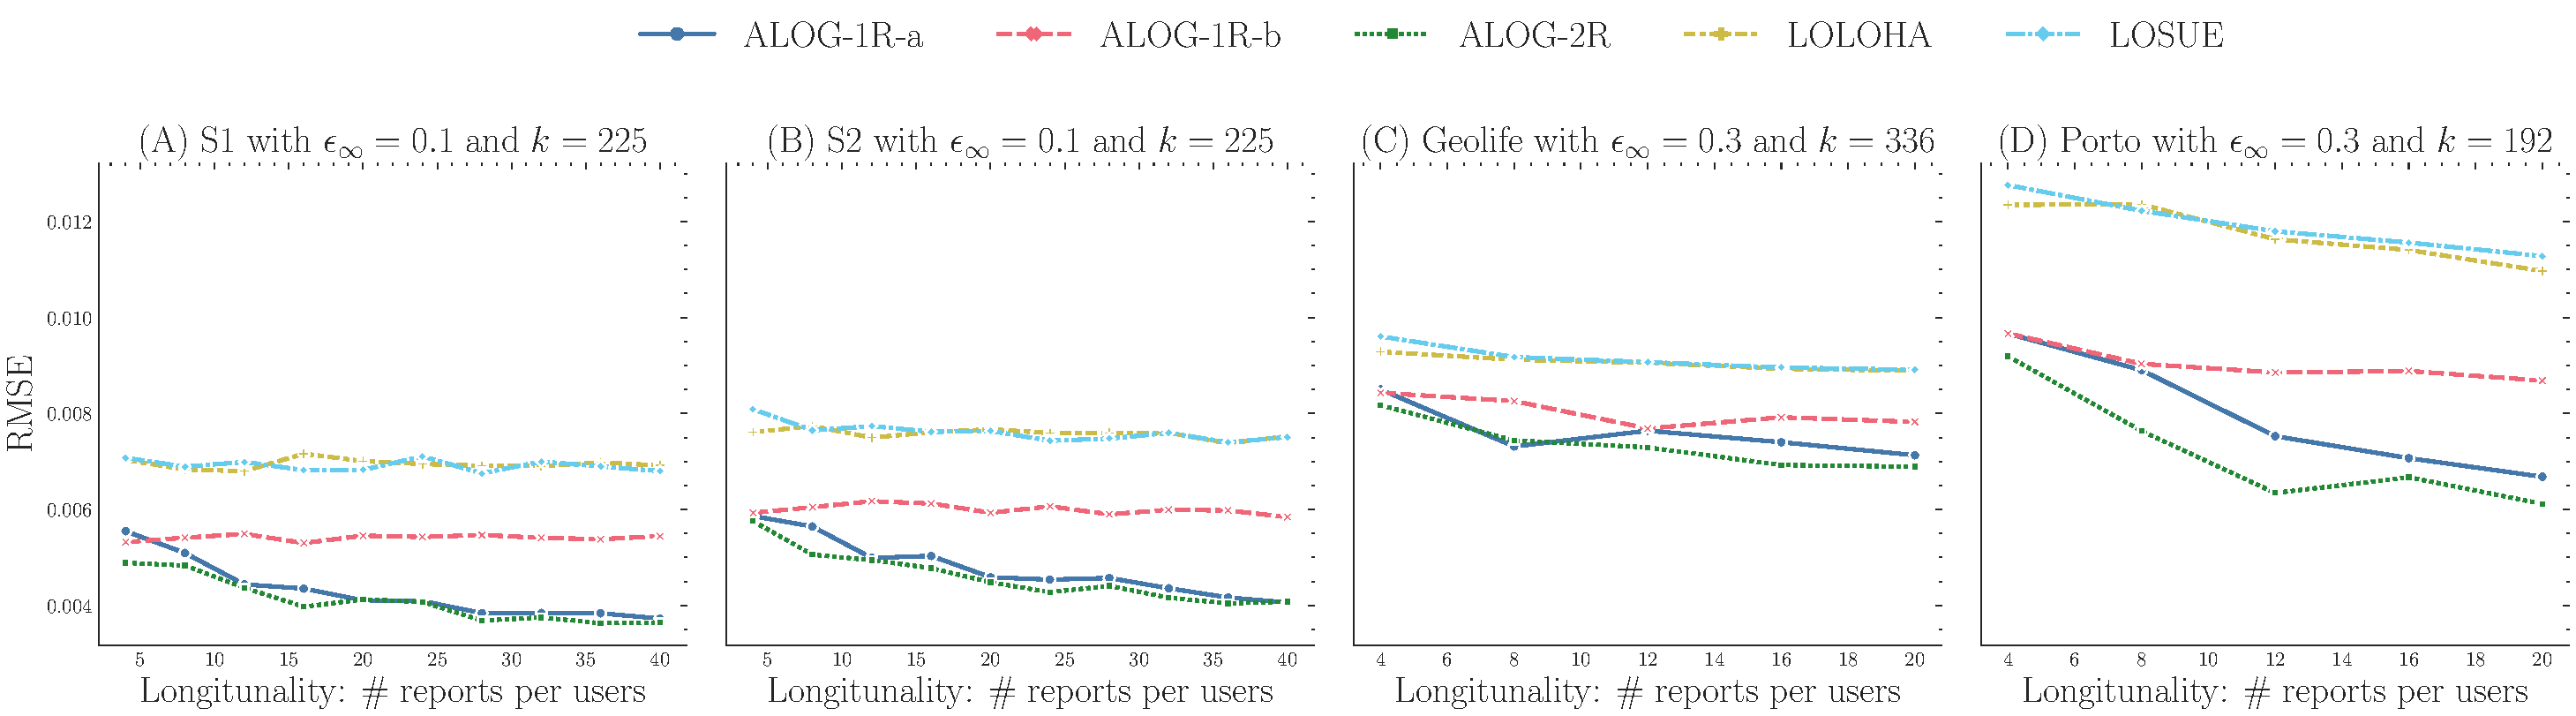
\includegraphics[width=\linewidth]{sections/figures/res_num_points.pdf}
    \caption{RMSE variation with the number of reports per user for the four datasets: S1, S2, GeoLife, and Porto.}
    \label{fig:longitudinality_barchart}
\end{figure*}

\paragraph{Budget Consumption:}we now begin a new analysis focusing on the budget privacy consumption. As shown in Table \ref{fig:bC_MSE}, the ALOG approaches demonstrate the highest budget consumption among the methods. This is expected since the grid adaptation process inherent to ALOG methods sacrifices a key efficiency mechanism available in other approaches: memoization. Memoization enables non-adaptive methods like LOLOHA, LOSUE, and RAPPOR to conserve the privacy budget by reusing previously computed information.

Despite this drawback, we now extend our analysis to explicitly evaluate privacy budget consumption using Pareto frontier analysis (Figure \ref{fig:res_pareto}). The Pareto frontiers reveal a clear efficiency-accuracy trade-off among the evaluated methods. Methods located closer to the frontier indicate superior performance, characterized by achieving lower RMSE at minimal budget consumption.

In the synthetic datasets, LOLOHA remains close to the frontier only under conditions of very low privacy budget consumption. In contrast, adaptive methods such as ALOG-2R and ALOG-1R-a dominate all other approaches at higher budget levels, consistently achieving lower RMSE values. For the GeoLife dataset, ALOG-2R and ALOG-1R-a outperform other methods starting from privacy budget consumptions above approximately $0.35$ and $0.29$, respectively. Similarly, for the Porto dataset, ALOG-1R-a dominates at budget consumptions exceeding $0.9$, whereas ALOG-2R surpasses all other methods once the budget exceeds $1.0$.

Non-adaptive methods, including LOLOHA, LOSUE, and RAPPOR, consistently demonstrate lower budget consumption due to memoization; however, their positions farther from the Pareto frontier clearly illustrate their limitations in accuracy compared to adaptive grid-based approaches.

\begin{figure*}[!tb]
    \centering
    \Description{budget paretto}
    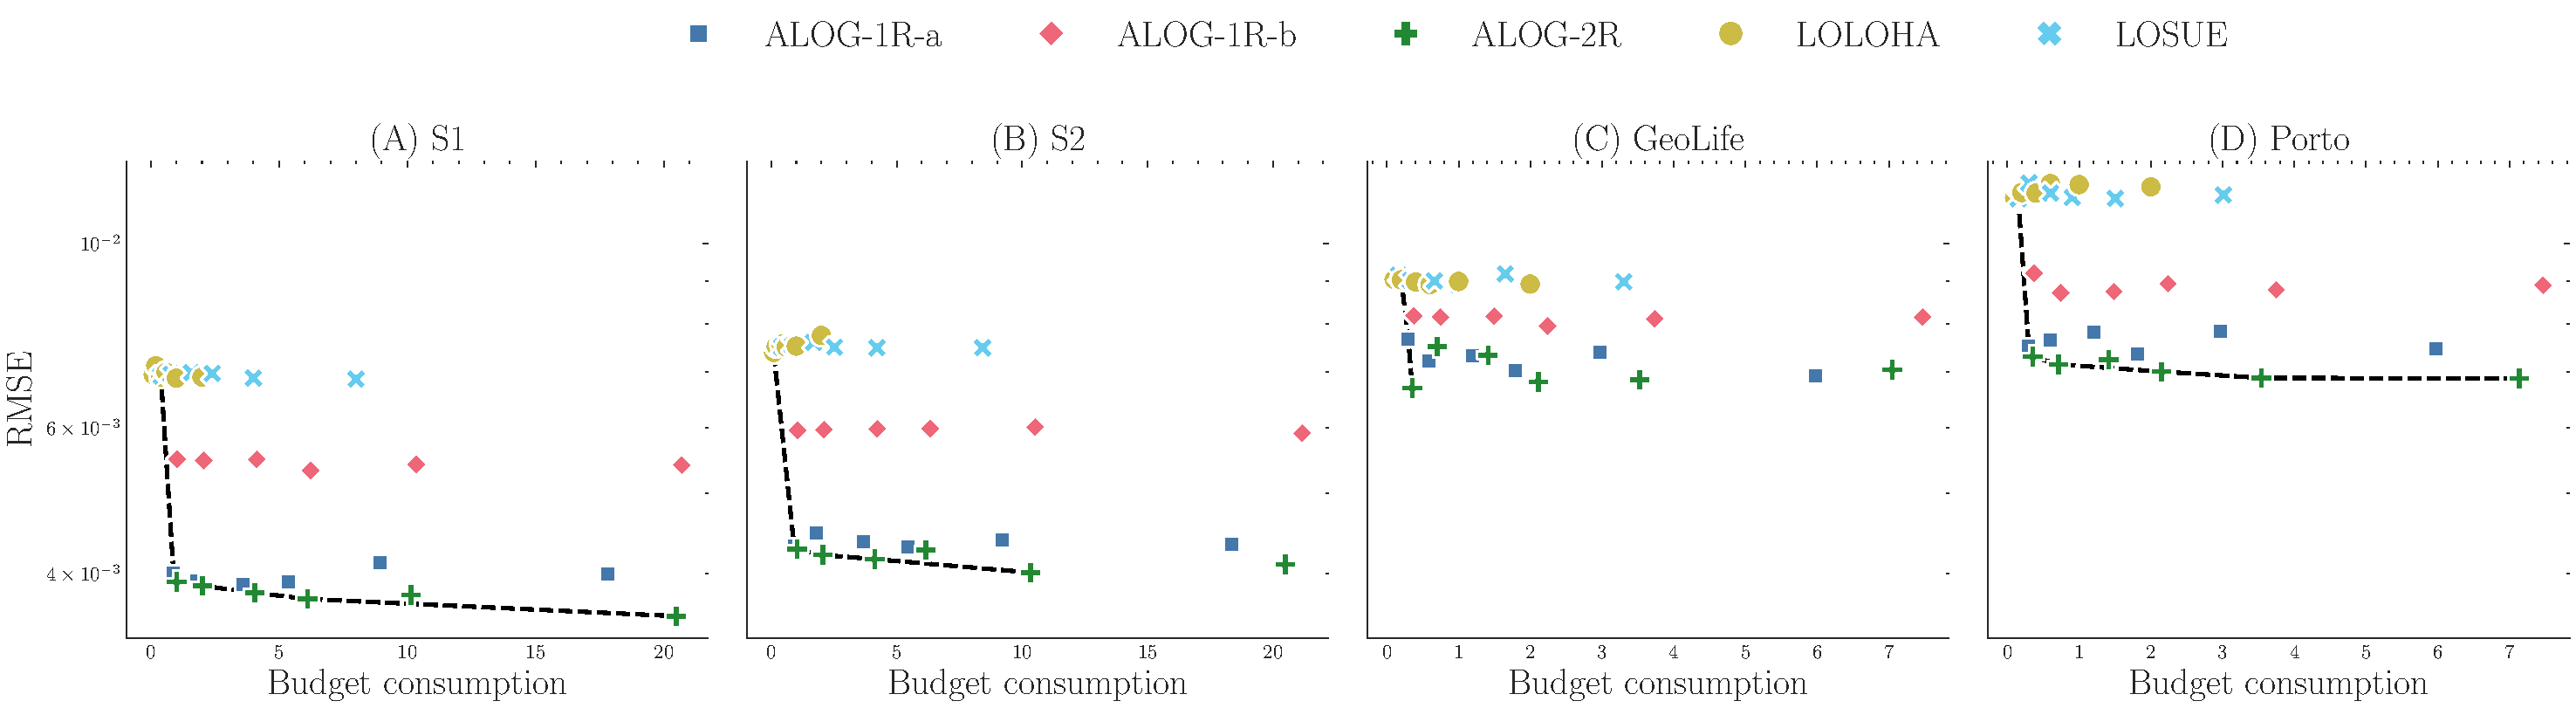
\includegraphics[width=\linewidth]{sections/figures/res_pareto.pdf}
    \caption{The Pareto frontier (black dashed line) demonstrates ALOG's superior trade-off between error (RMSE) and privacy budget consumption. Our method dominates the frontier in nearly all operational scenarios, establishing it as the preferred choice for most practical applications. Only in a narrow range of extremely low budget conditions does LOLOHA show marginally better performance.}
    \label{fig:res_pareto}
\end{figure*}

These results highlight that while ALOG approaches are more demanding in terms of budget consumption, their superior utility makes them highly advantageous for applications where accuracy and adaptability are critical, even in longitudinal settings.

% Non-adaptive methods, including LOLOHA, LOSUE, and RAPPOR, consistently demonstrate lower budget consumption due to memoization; however, their positions farther from the Pareto frontier clearly illustrate their limitations in accuracy compared to adaptive grid-based approaches. In contrast, while ALOG approaches are more demanding in terms of budget consumption, their superior utility, particularly in longitudinal settings, makes them highly advantageous for applications where accuracy and adaptability are critical.



% \begin{table*}[h!]
% \centering
% \small
% \caption{Budget Consumption for Datasets S1, S2, Geolife and Porto}
% \begin{tabular}{c|cccccc}
% \toprule
% \textbf{DataSet} & \textbf{ALOG-1R-a} & \textbf{ALOG-1R-b} & \textbf{ALOG-2R} & \textbf{LOLOHA} & \textbf{LOSUE} & \textbf{RAPPOR} \\
% \midrule
% S1 & \cellcolor{black!8}$\mathbf{1.78} $ & $2.07 $ & $2.02 $ & \cellcolor{black!8}$\mathbf{0.2}$ & $0.80$ & $0.80$ \\
% S2 & \cellcolor{black!8}$\mathbf{1.84} $ & $2.11 $ & $2.05 $ & \cellcolor{black!8}$\mathbf{0.2} $ & $0.84 $ & $0.86 $ \\
% Geolife & \cellcolor{black!8}$\mathbf{1.78} $ & $2.24 $ & $2.10 $ & \cellcolor{black!8}$\mathbf{0.59} $ & $0.99 $ & $0.99 $ \\
% Porto & \cellcolor{black!8}$\mathbf{1.78} $ & $2.07 $ & $2.02 $ & \cellcolor{black!8}$\mathbf{0.2}$ & $0.801$ & $0.801$ \\
% \bottomrule
% \end{tabular}
% \label{fig:bC_MSE}
% \end{table*}
% 
\begin{table}[!tb]
\centering
\footnotesize % or \footnotesize
\caption{Budget Consumption for Datasets S1, S2, Geolife and Porto}
\begin{tabular}{c|cccccc}
% \begin{tabularx}{\columnwidth}{@{}c|cccccc@{}}
% \begin{tabularx}{\columnwidth}{@{} L | C | C C C C C C @{}}
\toprule
\textbf{\makecell{DataSet}} & \textbf{\makecell{ALOG \\ 1R-a}} & \textbf{\makecell{ALOG \\ 1R-b}} & \textbf{\makecell{ALOG \\ 2R}} & \textbf{LOLOHA} & \textbf{LOSUE} & \textbf{RAPPOR} \\
\midrule
S1 & \cellcolor{black!8}$\mathbf{1.78} $ & $2.07 $ & $2.02 $ & \cellcolor{black!8}$\mathbf{0.2}$ & $0.80$ & $0.80$ \\
S2 & \cellcolor{black!8}$\mathbf{1.84} $ & $2.11 $ & $2.05 $ & \cellcolor{black!8}$\mathbf{0.2} $ & $0.84 $ & $0.86 $ \\
Geolife & \cellcolor{black!8}$\mathbf{1.78} $ & $2.24 $ & $2.10 $ & \cellcolor{black!8}$\mathbf{0.59} $ & $0.99 $ & $0.99 $ \\
Porto & \cellcolor{black!8}$\mathbf{1.78} $ & $2.07 $ & $2.02 $ & \cellcolor{black!8}$\mathbf{0.2}$ & $0.801$ & $0.801$ \\
\bottomrule
\end{tabular}
\label{fig:bC_MSE}
\end{table}
% 
\begin{figure*}[!ht]
    \centering
    \Description{window plots}
    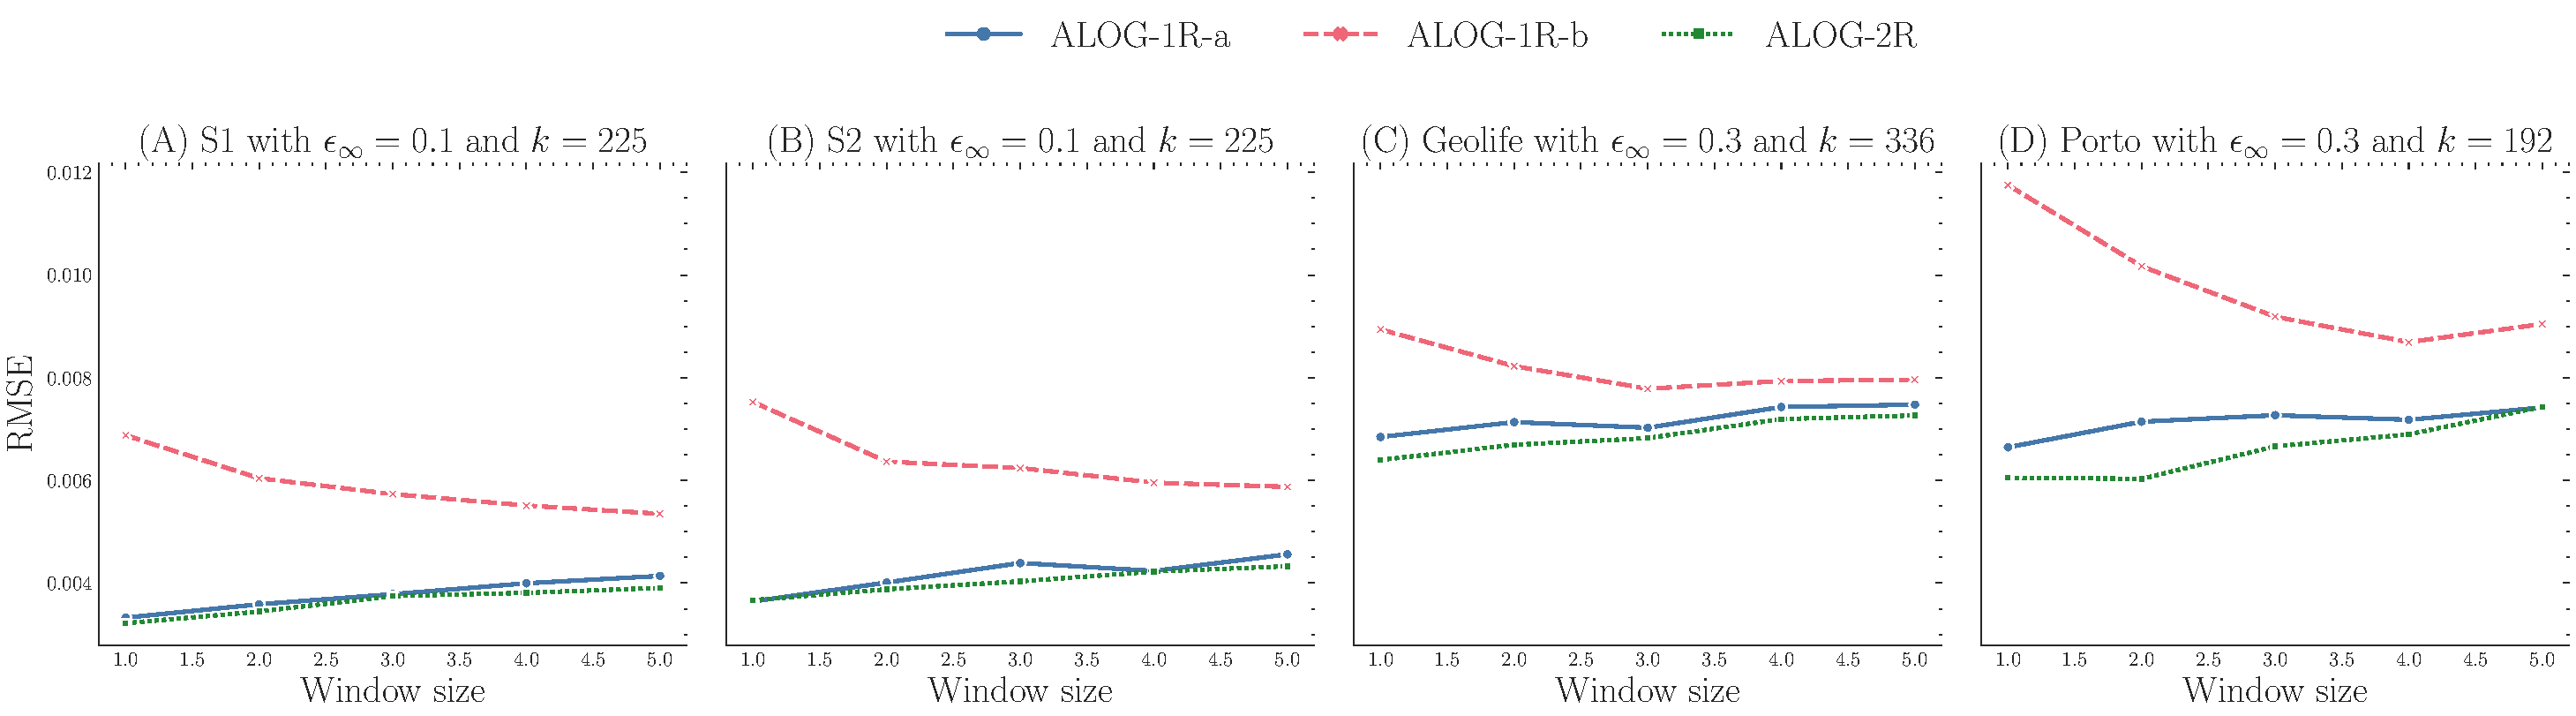
\includegraphics[width=\linewidth]{sections/figures/res_windows.pdf}
    \caption{RMSE variation in terms of the grid adaptation window size for the four datasets: S1, S2, GeoLife, and Porto.}
    \label{fig:Window_linechart}
\end{figure*}

\paragraph{GAW x Utility:}the grid adaptation window plays a crucial role in the performance of the ALOG approaches. Since all three ALOG variants consistently outperform uniform grid approaches, it is essential to understand their behavior in terms of grid size and how it affects their utility.

Figure \ref{fig:Window_linechart} illustrates that ALOG-2R and ALOG-1R-a maintain better utility across all tested window sizes for each dataset. However, a notable trend emerges: as the window size increases, the error for ALOG-2R and ALOG-1R-a also increases. Conversely, ALOG-1R-b demonstrates a decreasing error trend as the window size grows. This divergence arises from the distinct grid adaptation mechanisms employed by these approaches.

ALOG-1R-a and ALOG-2R experience an increase in error with larger window sizes primarily due to their reliance on the previous grid for adaptation. These methods dynamically split grid cells to increase granularity when needed but lack the ability to reduce granularity by merging cells as data density decreases. This limitation becomes more pronounced as the window size grows because larger windows lead to greater variations in data distribution over time. The inability to decrease granularity hinders their ability to adjust effectively to these abrupt changes, resulting in inefficiencies and increased error.

In contrast, ALOG-1R-b demonstrates better performance in scenarios with larger window sizes due to its use of a fixed base grid during the adaptation process. This design allows ALOG-1R-b to reset and adjust more effectively to significant changes in data distribution, making it more resilient to abrupt shifts that occur when the window size is larger. By avoiding reliance on a previous grid, ALOG-1R-b can maintain alignment with current data density, ensuring more consistent and efficient performance even under challenging conditions. This highlights the importance of adaptability in handling varying data dynamics, particularly in scenarios with large adaptation windows.

In summary, the increasing error trend for ALOG-2R and ALOG-1R-a with larger window sizes is a consequence of their grid adaptation process, which cannot shrink the grid when necessary. ALOG-1R-b, with its reliance on a base grid, provides better adjustment and resilience to data dynamics over longer periods, highlighting the trade-offs inherent in these adaptive strategies.


% \begin{figure*}[!ht]
%     \centering
%     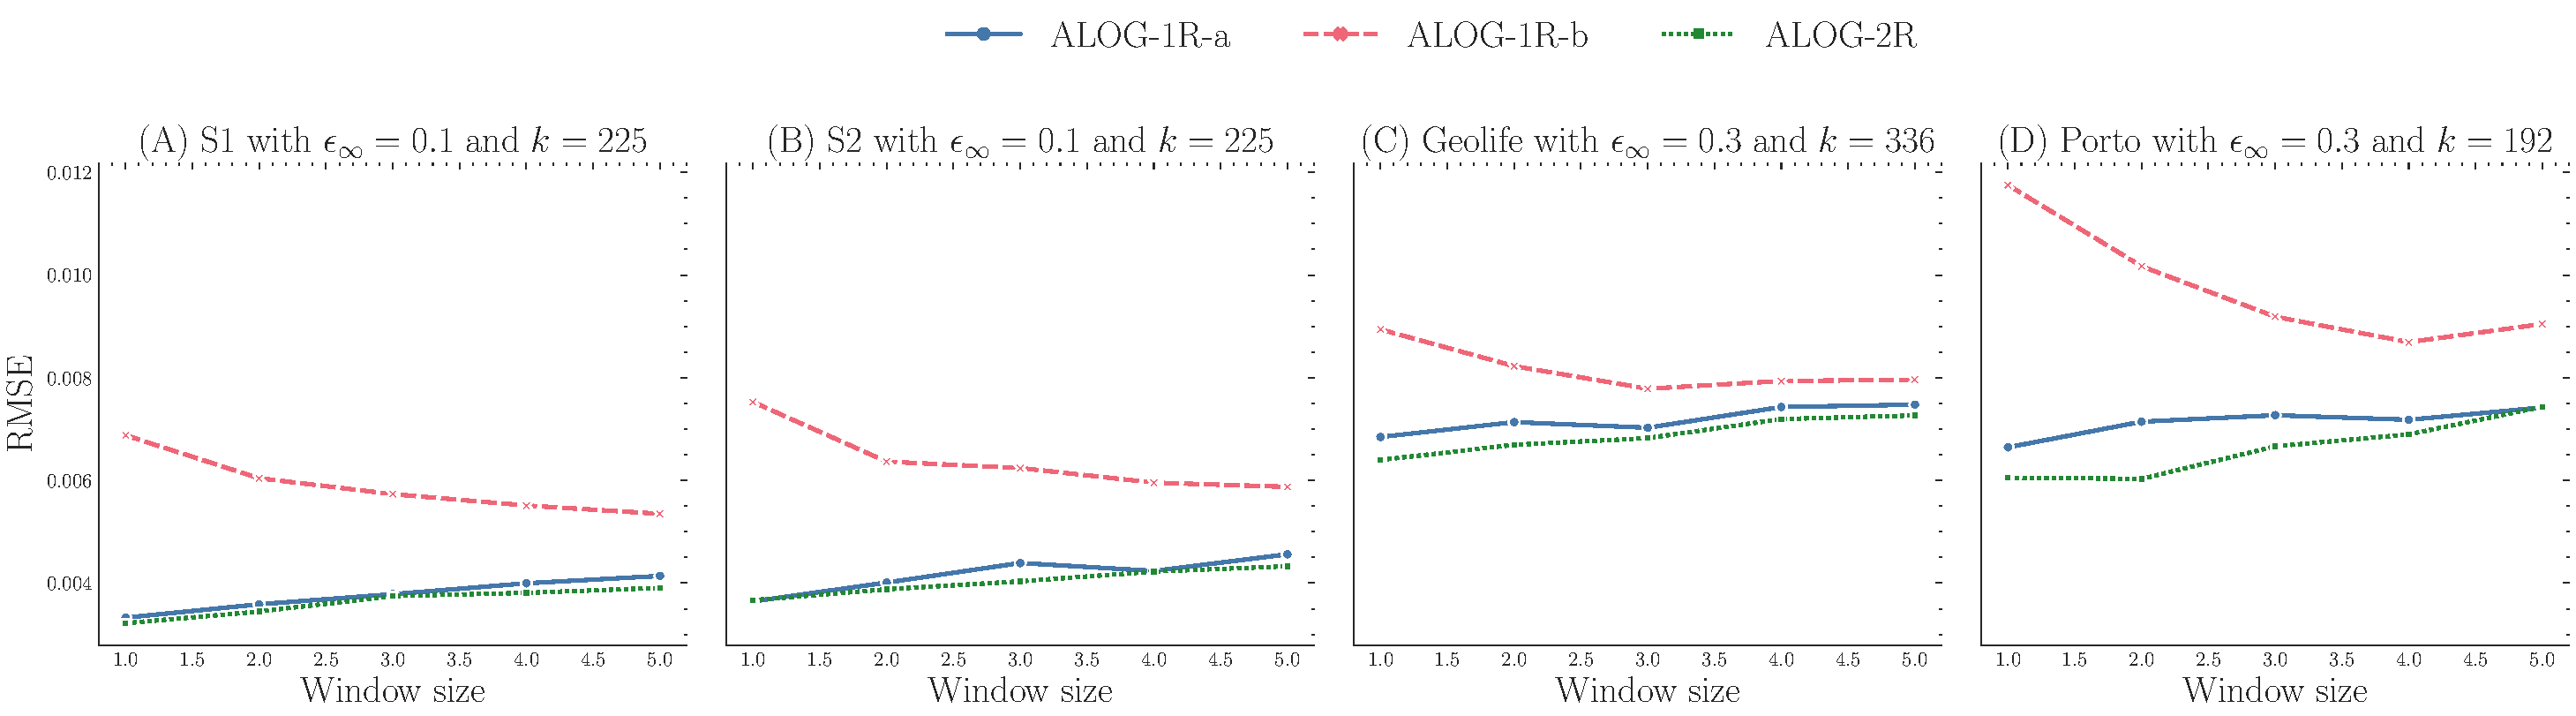
\includegraphics[width=\linewidth]{sections/figures/res_windows.pdf}
%     \caption{RMSE variation in terms of the grid adaptation window size for the four datasets: S1, S2, GeoLife, and Porto.}
%     \label{fig:Window_linechart}
% \end{figure*}


\paragraph{Budget partition x Utility:}The final aspect of our analysis focuses on ALOG-2R, the best-performing method across datasets. A critical factor influencing its performance is the partitioning of the privacy budget between the first and second rounds. This partitioning directly affects the utility achieved by ALOG-2R, as it determines the extent to which each round can contribute to the grid's adaptability and the accuracy of the results.

In the first round, the budget is primarily used to initialize the grid structure and adapt it to the data distribution. This stage is crucial for ensuring that the grid reflects the overall data density and establishes a strong foundation for further refinements. The second round leverages the remaining budget to refine the grid further and address more localized variations in the data.

Table \ref{tab:bpmse} reveals that for datasets S1, S2, and Porto, the optimal partitioning allocates 30\% of the total budget to the first round, with the remaining 70\% allocated to the second round. This configuration ensures sufficient budget for initializing the grid while allowing for meaningful refinements in the second round.

Conversely, the Geolife dataset exhibits only minor differences in RMSE across the tested budget partitioning strategies. The optimal configuration, with 50\% of the budget assigned to each of the two allocation stages, results in a minimal improvement in RMSE. This suggests that the specific characteristics of the Geolife data permit a wider range of effective privacy budget distributions.
% 
\begin{table}[!tb]
\centering
\footnotesize
\caption{RMSE as a function of budget proportion used in ALOG-2R for rounds 1 and 2 (values are in units of $\times 10^{-3}$)}
\begin{tabular}{c|cccccc}
\toprule
\textbf{DataSet} & \textbf{S1} & \textbf{S2} & \textbf{Geolife} & \textbf{Porto} \\
\midrule
$\mathbf{(r_1=0.1\epsilon,r_2=0.9\epsilon)}$ & $3.88$ & $4.18 $ & $7.07 $ & $6.96$\\
$\mathbf{(r_1=0.3\epsilon,r_2=0.7\epsilon)}$ & \cellcolor{black!8}$\mathbf{3.82} $ & \cellcolor{black!8}$\mathbf{4.06} $ & $7.07 $ & \cellcolor{black!8}$\mathbf{6.87}$ \\
$\mathbf{(r_1=0.5\epsilon,r_2=0.5\epsilon)}$ & $3.92 $ & $4.08 $ & \cellcolor{black!8}$\mathbf{7.06} $ & $7.08 $ \\
$\mathbf{(r_1=0.7\epsilon,r_2=0.3\epsilon)}$ & $3.87$ & $4.12 $ & $7.07$ & $7.39$ \\
\bottomrule
\end{tabular}
\label{tab:bpmse}
\end{table}
% 
In summary, the results emphasize the robustness of ALOG-2R in delivering superior utility through its adaptive grid mechanism, making it a strong candidate for practical applications in privacy-preserving data analysis. The findings also underscore the importance of tuning parameters such as grid adaptation windows and budget partitioning to maximize performance across varying scenarios.

